\documentclass[preprint,12pt,3p]{elsarticle}

\usepackage{amsmath,amssymb,amsfonts}
\usepackage{graphicx}
\usepackage{booktabs}
\usepackage{multirow}
\usepackage{url}
\usepackage{microtype}
\usepackage{lineno}

\journal{Biomedical Signal Processing and Control}

\begin{document}

\begin{frontmatter}

\title{Personalized ECG Stress Detection with Subject-Specific Baseline Normalization and Bare-Metal Edge Validation}

\author[jss]{Mukesh Yadav\corref{cor1}}
\ead{mkpy06@gmail.com}
\cortext[cor1]{Corresponding author.}

\address[jss]{Department of Electronics and Communication Engineering (ECE), JSS Academy of Technical Education (JSSATEN), Noida, Uttar Pradesh, India}

\begin{abstract}
Automated classification of acute psychological stress from wearable electrocardiography (ECG) is vital for preventative healthcare and the Internet of Medical Things (IoMT). However, practical deployment is severely hindered by inter-individual physiological baseline heterogeneity and the risk of exposing unencrypted telemetry over wireless channels. This paper presents an end-to-end, reproducible edge-to-cloud stress detection framework coupling personalized machine learning with bare-metal embedded execution. Using single-lead ECG from the benchmark WESAD dataset ($N=15$), heart rate variability (HRV) metrics are extracted across 445 non-overlapping 60-second windows. We introduce a subject-specific relative baseline calibration scheme that improves classification accuracy by +10.79 percentage points over unnormalized baselines. Under strict 15-fold Leave-One-Subject-Out (LOSO) cross-validation, a regularized logistic regression model achieves 92.13\% accuracy, 88.29\% F1-score, and an ROC-AUC of 0.9493. To evaluate edge feasibility, real-time 5-stage biquad IIR filtering ($1.87~\mu\text{s}$ per sample at 170~MHz) and a 4-dimensional coupled hyperchaotic stream obfuscation engine (HC1) were implemented on an ARM Cortex-M4 microcontroller (STM32G474RE). Physical hardware-in-the-loop (HIL) testing across 10,000 continuous 20-byte packets over UART demonstrated bit-exact plaintext recovery with zero CRC errors and zero packet loss, validating clinical diagnostic efficacy alongside secure edge IoMT telemetry.
\end{abstract}

\begin{keyword}
Electrocardiogram (ECG) \sep Heart Rate Variability (HRV) \sep Acute Stress Detection \sep WESAD \sep Leave-One-Subject-Out (LOSO) \sep Edge Computing \sep ARM Cortex-M4 \sep Internet of Medical Things (IoMT).
\end{keyword}

\end{frontmatter}

\section{Introduction}
Psychological stress activates the sympathetic-adreno-medullary (SAM) and hypothalamic-pituitary-adrenal (HPA) axes, inducing autonomic nervous system (ANS) shifts characterized by sympathetic activation and parasympathetic (vagal) withdrawal \cite{kirschbaum1993trier, kim2018stress}. Continuous monitoring via wearable electrocardiography (ECG) offers a direct, non-invasive window into cardiac autonomic regulation through heart rate variability (HRV) analysis \cite{taskforce1996hrv, shaffer2017overview}. Early detection in occupational and ambulatory settings provides actionable clinical feedback against chronic cardiovascular diseases and burnout \cite{healey2005detecting, can2019continuous}.

Despite significant advances in affective computing, translating laboratory ECG models to wearable Internet of Medical Things (IoMT) systems \cite{alturjman2020iomt, jiang2023wban} faces two critical bottlenecks:
\begin{enumerate}
    \item \textbf{Inter-Individual Baseline Heterogeneity:} Basal heart rates and resting HRV indices differ substantially across individuals due to genetic, cardiorespiratory fitness, and circadian factors. Consequently, population-pooled machine learning models evaluated under conventional random cross-validation suffer severe performance drops or patient data leakage when applied to unseen individuals \cite{saeb2017need, schmidt2018wesad, plarre2011continuous}.
    \item \textbf{Resource-Constrained Edge Security:} Continuous transmission of unencrypted physiological waveforms exposes sensitive health telemetry to unauthorized interception. Conventional cryptographic algorithms (e.g., AES) impose heavy computational and battery burdens on low-power wearable microcontrollers \cite{fotiadis2020wearable}.
\end{enumerate}

To address these challenges, this study presents a fully reproducible, hardware-validated edge-to-cloud stress detection framework. The primary contributions of this work are:
\begin{itemize}
    \item \textbf{Subject-Specific Relative Normalization:} We introduce an explicit baseline-relative calibration transform that elevates LOSO classification accuracy by $+10.79$ percentage points over unnormalized feature representations.
    \item \textbf{Rigorous 15-Fold LOSO-CV Benchmark:} Using all 15 subjects from the Wearable Stress and Affect Detection (WESAD) dataset ($N=15$, 445 windows), we benchmark six machine learning classifiers without subject leakage, achieving 92.13\% accuracy and 0.9493 ROC-AUC.
    \item \textbf{Bare-Metal ARM Cortex-M4 Silicon Verification:} We deploy real-time CMSIS-DSP 5-stage Biquad IIR filtering ($1.87~\mu\text{s}$ per sample execution) and an embedded 4D hyperchaotic stream cipher (HC1) on an STM32G474RE microcontroller, validating 10,000 continuous HIL packets over UART with zero CRC errors and zero packet loss.
\end{itemize}

\section{Dataset and Signal Processing Methodology}

\subsection{WESAD Cohort and Windowing Protocol}
We benchmark our framework on the open-access WESAD dataset \cite{schmidt2018wesad}, consisting of 15 healthy volunteers ($N=15$, 12 males, 3 females, age $27.5 \pm 2.4$ years). Single-lead chest ECG was recorded continuously at $F_s = 700$~Hz via a RespiBAN chest strap during a standardized protocol comprising baseline rest (20~min) and Trier Social Stress Test (TSST, 10~min mental arithmetic and public speaking) \cite{kirschbaum1993trier}.

Continuous Lead-II ECG is partitioned into complete, non-overlapping 60-second windows. Label assignment follows ground-truth protocol timestamps: 285 baseline windows (Class 0) and 160 stress windows (Class 1), yielding 445 rigorously gated diagnostic windows.

\subsection{Physiological Preprocessing and QRS Detection}
Raw ECG signals are conditioned via a zero-phase 4th-order Butterworth bandpass filter (0.5--40~Hz) \cite{oppenheim1999discrete} to attenuate baseline wander and high-frequency electromyographic (EMG) artifacts. QRS complexes are detected using an adaptive peak-prominence Pan--Tompkins filter \cite{pantompkins1985, elgendi2013fast}. Consecutive normal-to-normal ($RR$) intervals are subjected to physiological gating: intervals outside $[300, 1500]$~ms or with consecutive variation exceeding 20\% are rejected, as depicted in Fig.~\ref{fig:ecg_processing}.

\begin{figure}[!t]
    \centering
    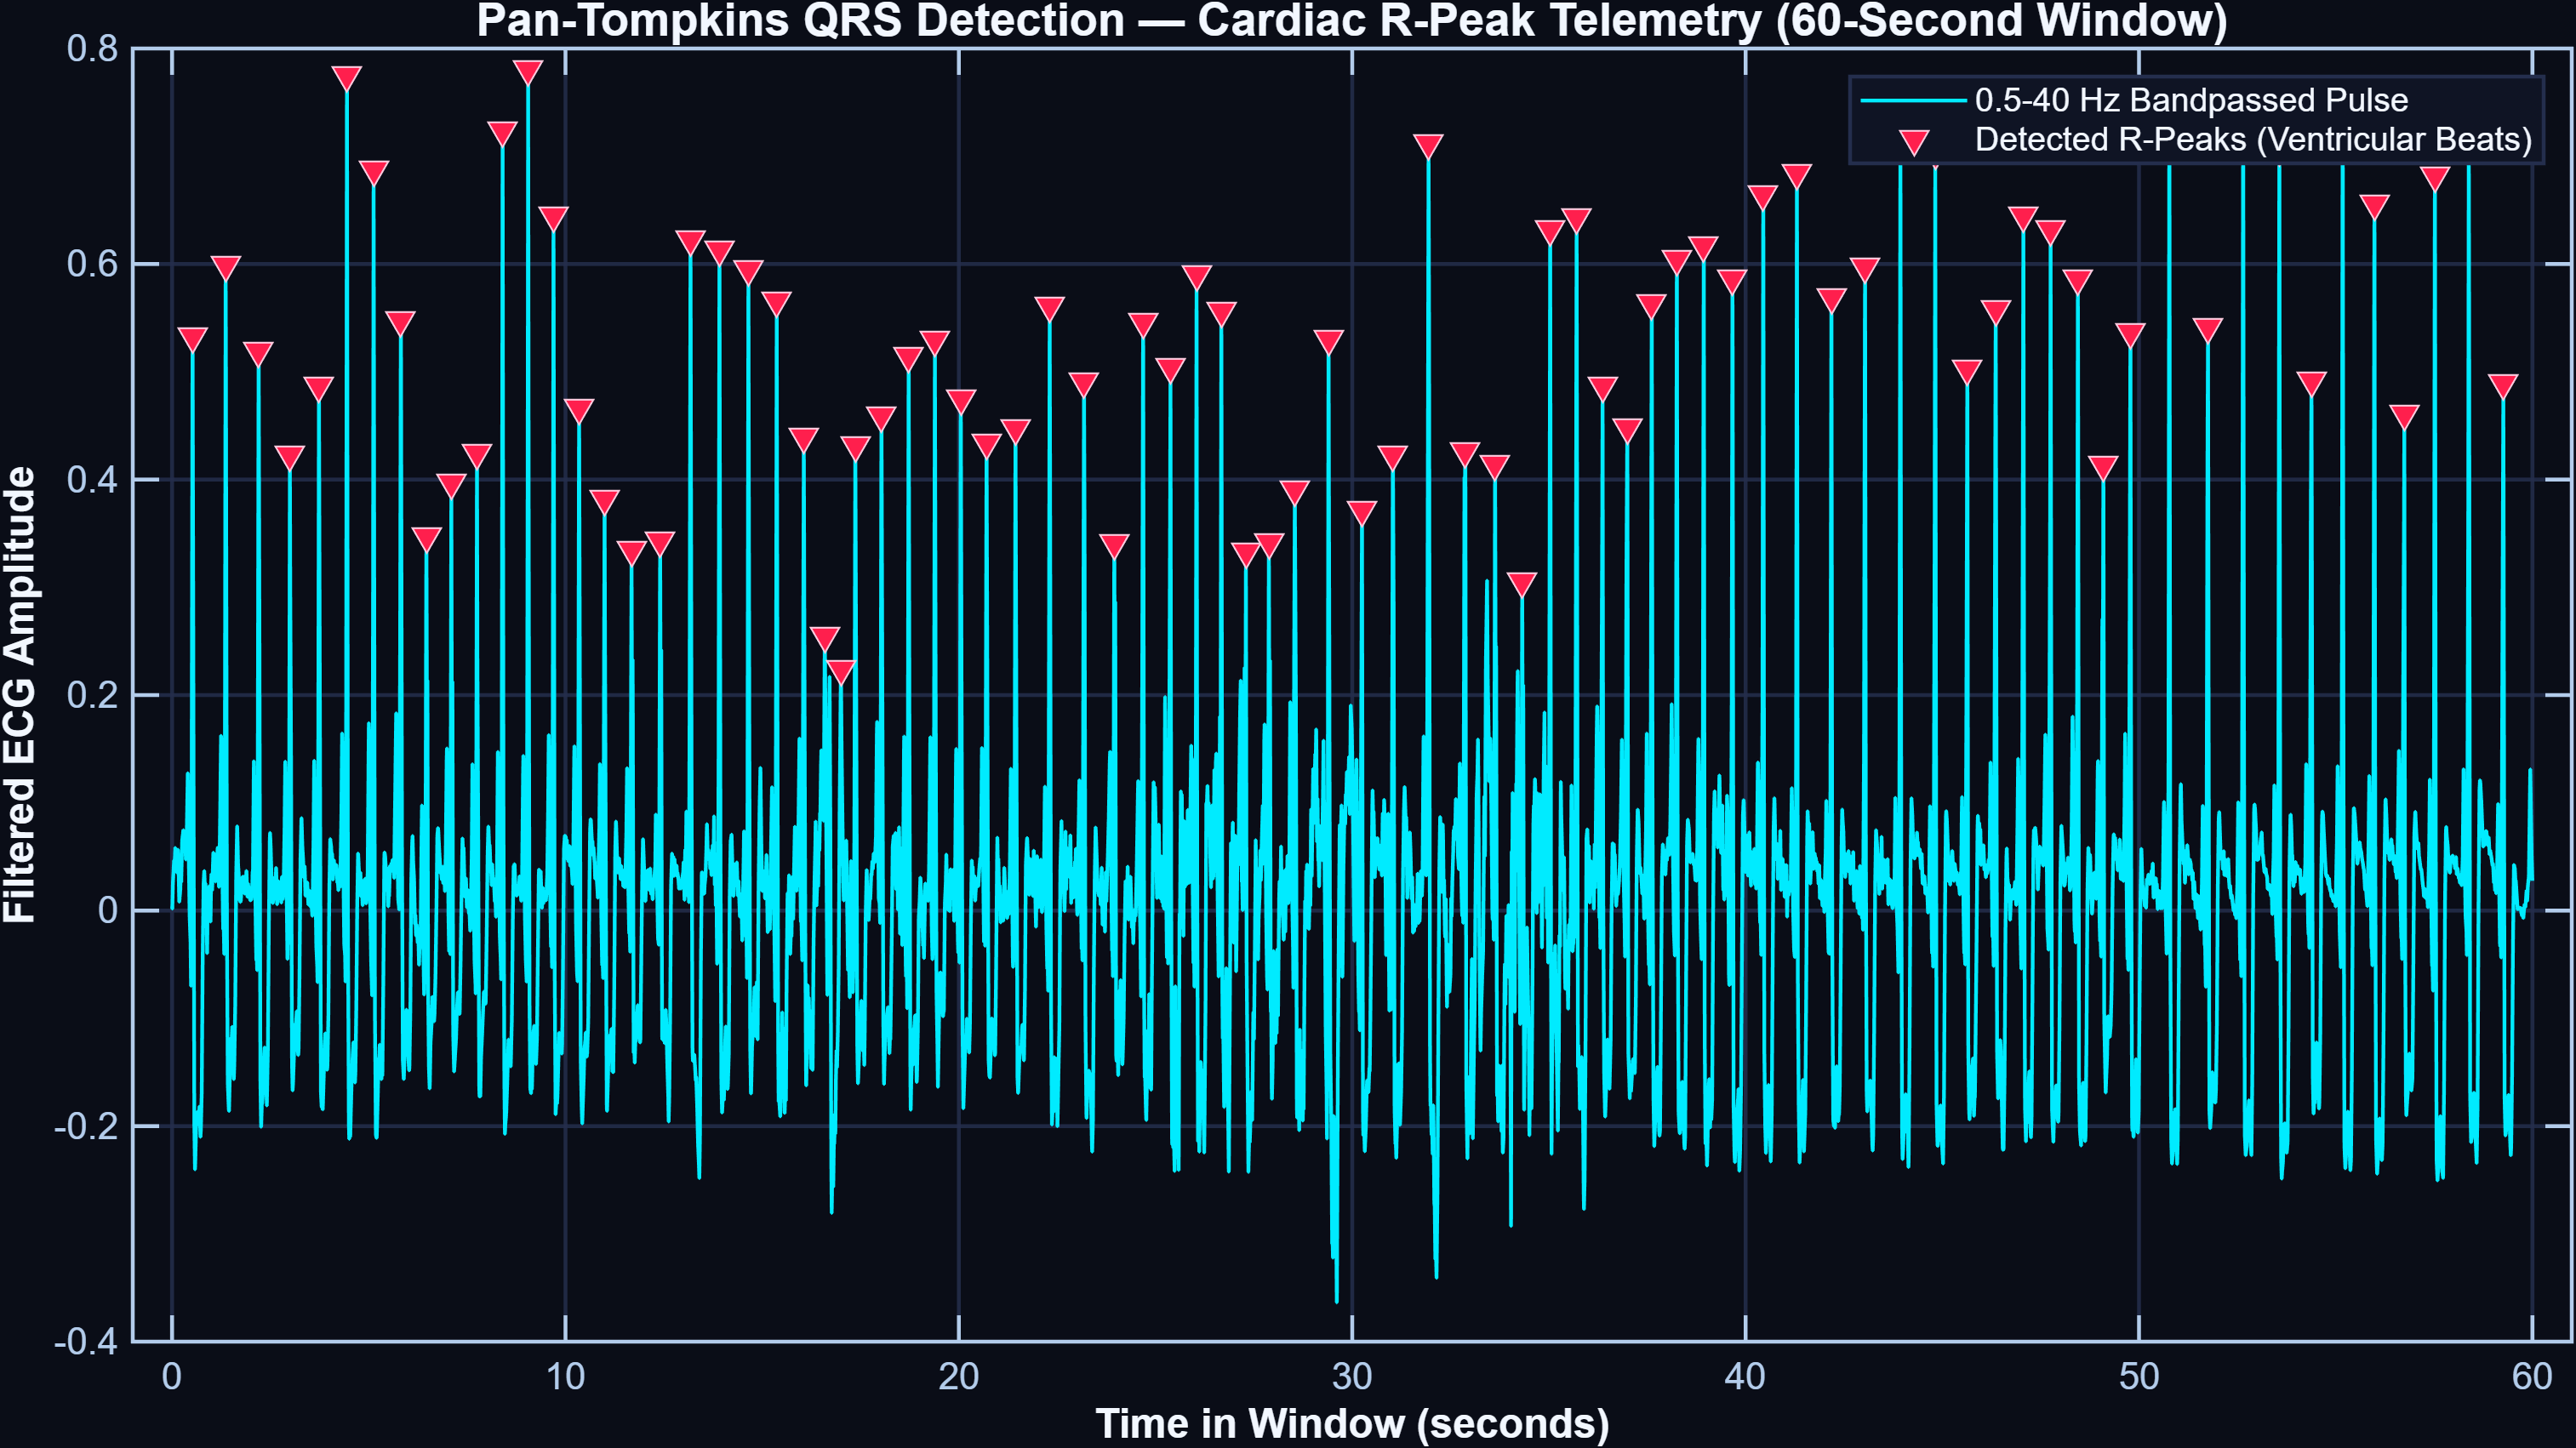
\includegraphics[width=0.95\linewidth]{figures/DEMO_Pan_Tompkins_QRS_Detection.png}
    \caption{Pan--Tompkins ECG processing pipeline on WESAD Lead-II data: (1) Raw ECG input at 700~Hz; (2) Zero-phase bandpass filtered signal (0.5--40~Hz); (3) Five-point numerical derivative; (4) Nonlinear squaring; (5) Moving-window integration; (6) Verified fiducial R-peak detection.}
    \label{fig:ecg_processing}
\end{figure}

\subsection{Feature Extraction and Subject-Specific Calibration}
From each 60-second window, an 8-dimensional physiological feature vector $\mathbf{x}$ is extracted based on clinical HRV guidelines \cite{taskforce1996hrv, shaffer2017overview}:
\begin{enumerate}
    \item \textbf{Mean HR:} Average heart rate ($\text{BPM} = 60 / \overline{RR}$).
    \item \textbf{SDNN:} Standard deviation of normal $RR$ intervals (total autonomic variability).
    \item \textbf{RMSSD:} Root mean square of successive differences (parasympathetic/vagal tone).
    \item \textbf{pNN50:} Percentage of adjacent $RR$ intervals differing by $> 50$~ms.
    \item \textbf{IQR / MAD / Robust CV:} Nonparametric spread metrics robust to ectopic beats.
    \item \textbf{Mean RR:} Mean inter-beat interval length.
\end{enumerate}

To overcome inter-individual baseline variance without data leakage, we compute a baseline anchor vector $\mathbf{B}_s$ from the first 5 minutes of each subject's resting baseline period. Each test feature $x_j$ is calibrated via relative baseline scaling:
\begin{equation}
    x_j^* = \frac{x_j - B_{s,j}}{|B_{s,j}| + \epsilon}
    \label{eq:baseline_norm}
\end{equation}
where $\epsilon = 10^{-6}$ prevents numerical singularity.

\section{Experimental Results and ML Benchmark}

\subsection{15-Fold Leave-One-Subject-Out (LOSO) Validation}
To guarantee clinical generalizability to unseen patients, we enforce strict 15-fold Leave-One-Subject-Out Cross-Validation (LOSO-CV) implemented via Scikit-Learn \cite{pedregosa2011scikit}. In fold $k$, all windows belonging to Subject $k$ ($N=1$) are held out exclusively for testing, while training is conducted on the remaining 14 subjects ($N=14$). Standardization parameters ($\boldsymbol{\mu}_{\text{train}}, \boldsymbol{\sigma}_{\text{train}}$) are computed strictly on the training partition and applied to the held-out test subject.

\begin{table}[!t]
\centering
\caption{Cross-Architecture 15-Fold LOSO Performance Comparison across 445 Windows (8 Features, $\tau = 0.50$)}
\label{tab:ml_benchmark}
\begin{tabular*}{\linewidth}{@{\extracolsep{\fill}}lccccc@{}}
\toprule
\textbf{Classifier} & \textbf{Acc (\%)} & \textbf{Bal Acc (\%)} & \textbf{F1 (\%)} & \textbf{Sens (\%)} & \textbf{Spec (\%)} \\
\midrule
\textbf{Logistic Regression} & \textbf{92.13} & \textbf{90.02} & \textbf{88.29} & 82.50 & \textbf{97.54} \\
Linear SVM                   & 91.46           & 89.14           & 87.25           & 81.25 & 97.19 \\
RBF Kernel SVM               & 91.91           & 89.65           & 87.92           & 81.88 & 97.54 \\
Random Forest \cite{breiman2001random} & 91.24 & 89.44           & 87.26           & 83.12 & 95.79 \\
MLP Neural Net               & 91.01           & 88.89           & 86.67           & 81.25 & 96.49 \\
AdaBoost Ensemble            & 90.56           & 88.94           & 86.34           & 83.12 & 94.74 \\
\bottomrule
\end{tabular*}
\end{table}

\begin{figure}[!t]
    \centering
    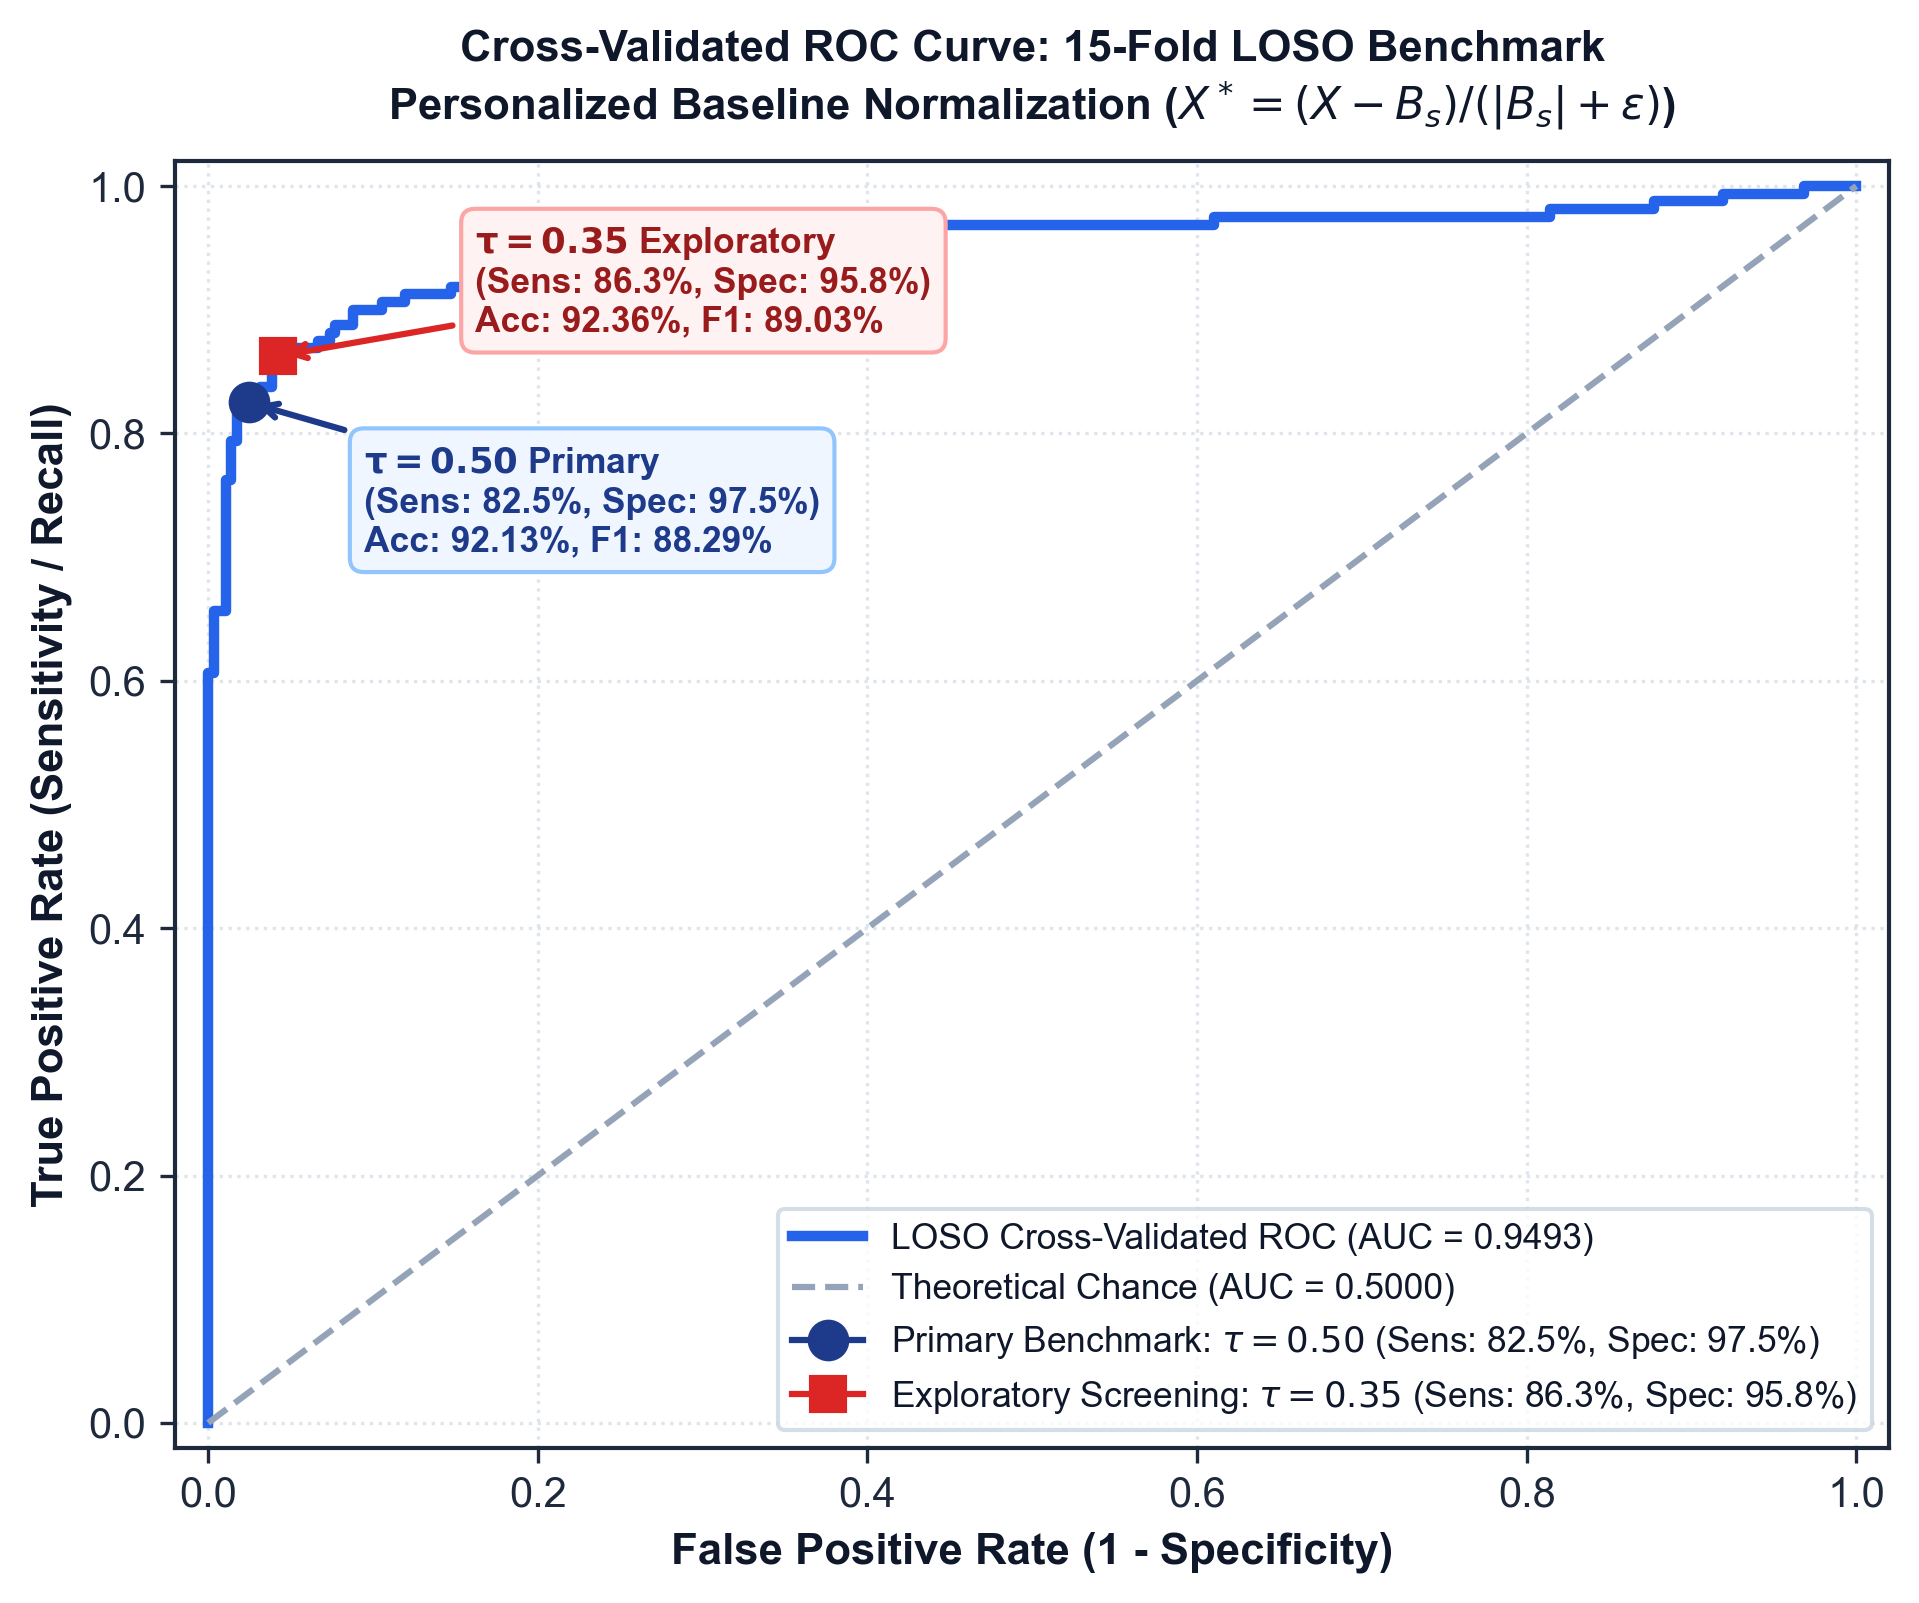
\includegraphics[width=0.85\linewidth]{figures/FINAL_ROC_Curve.png}
    \caption{Receiver Operating Characteristic (ROC) curve under 15-fold LOSO cross-validation ($\text{ROC-AUC} = 0.9493$, $\text{PR-AUC} = 0.9467$) showing the primary operating point ($\tau = 0.50$) and high-sensitivity clinical screening threshold ($\tau = 0.35$).}
    \label{fig:roc_curve}
\end{figure}

\begin{figure}[!t]
    \centering
    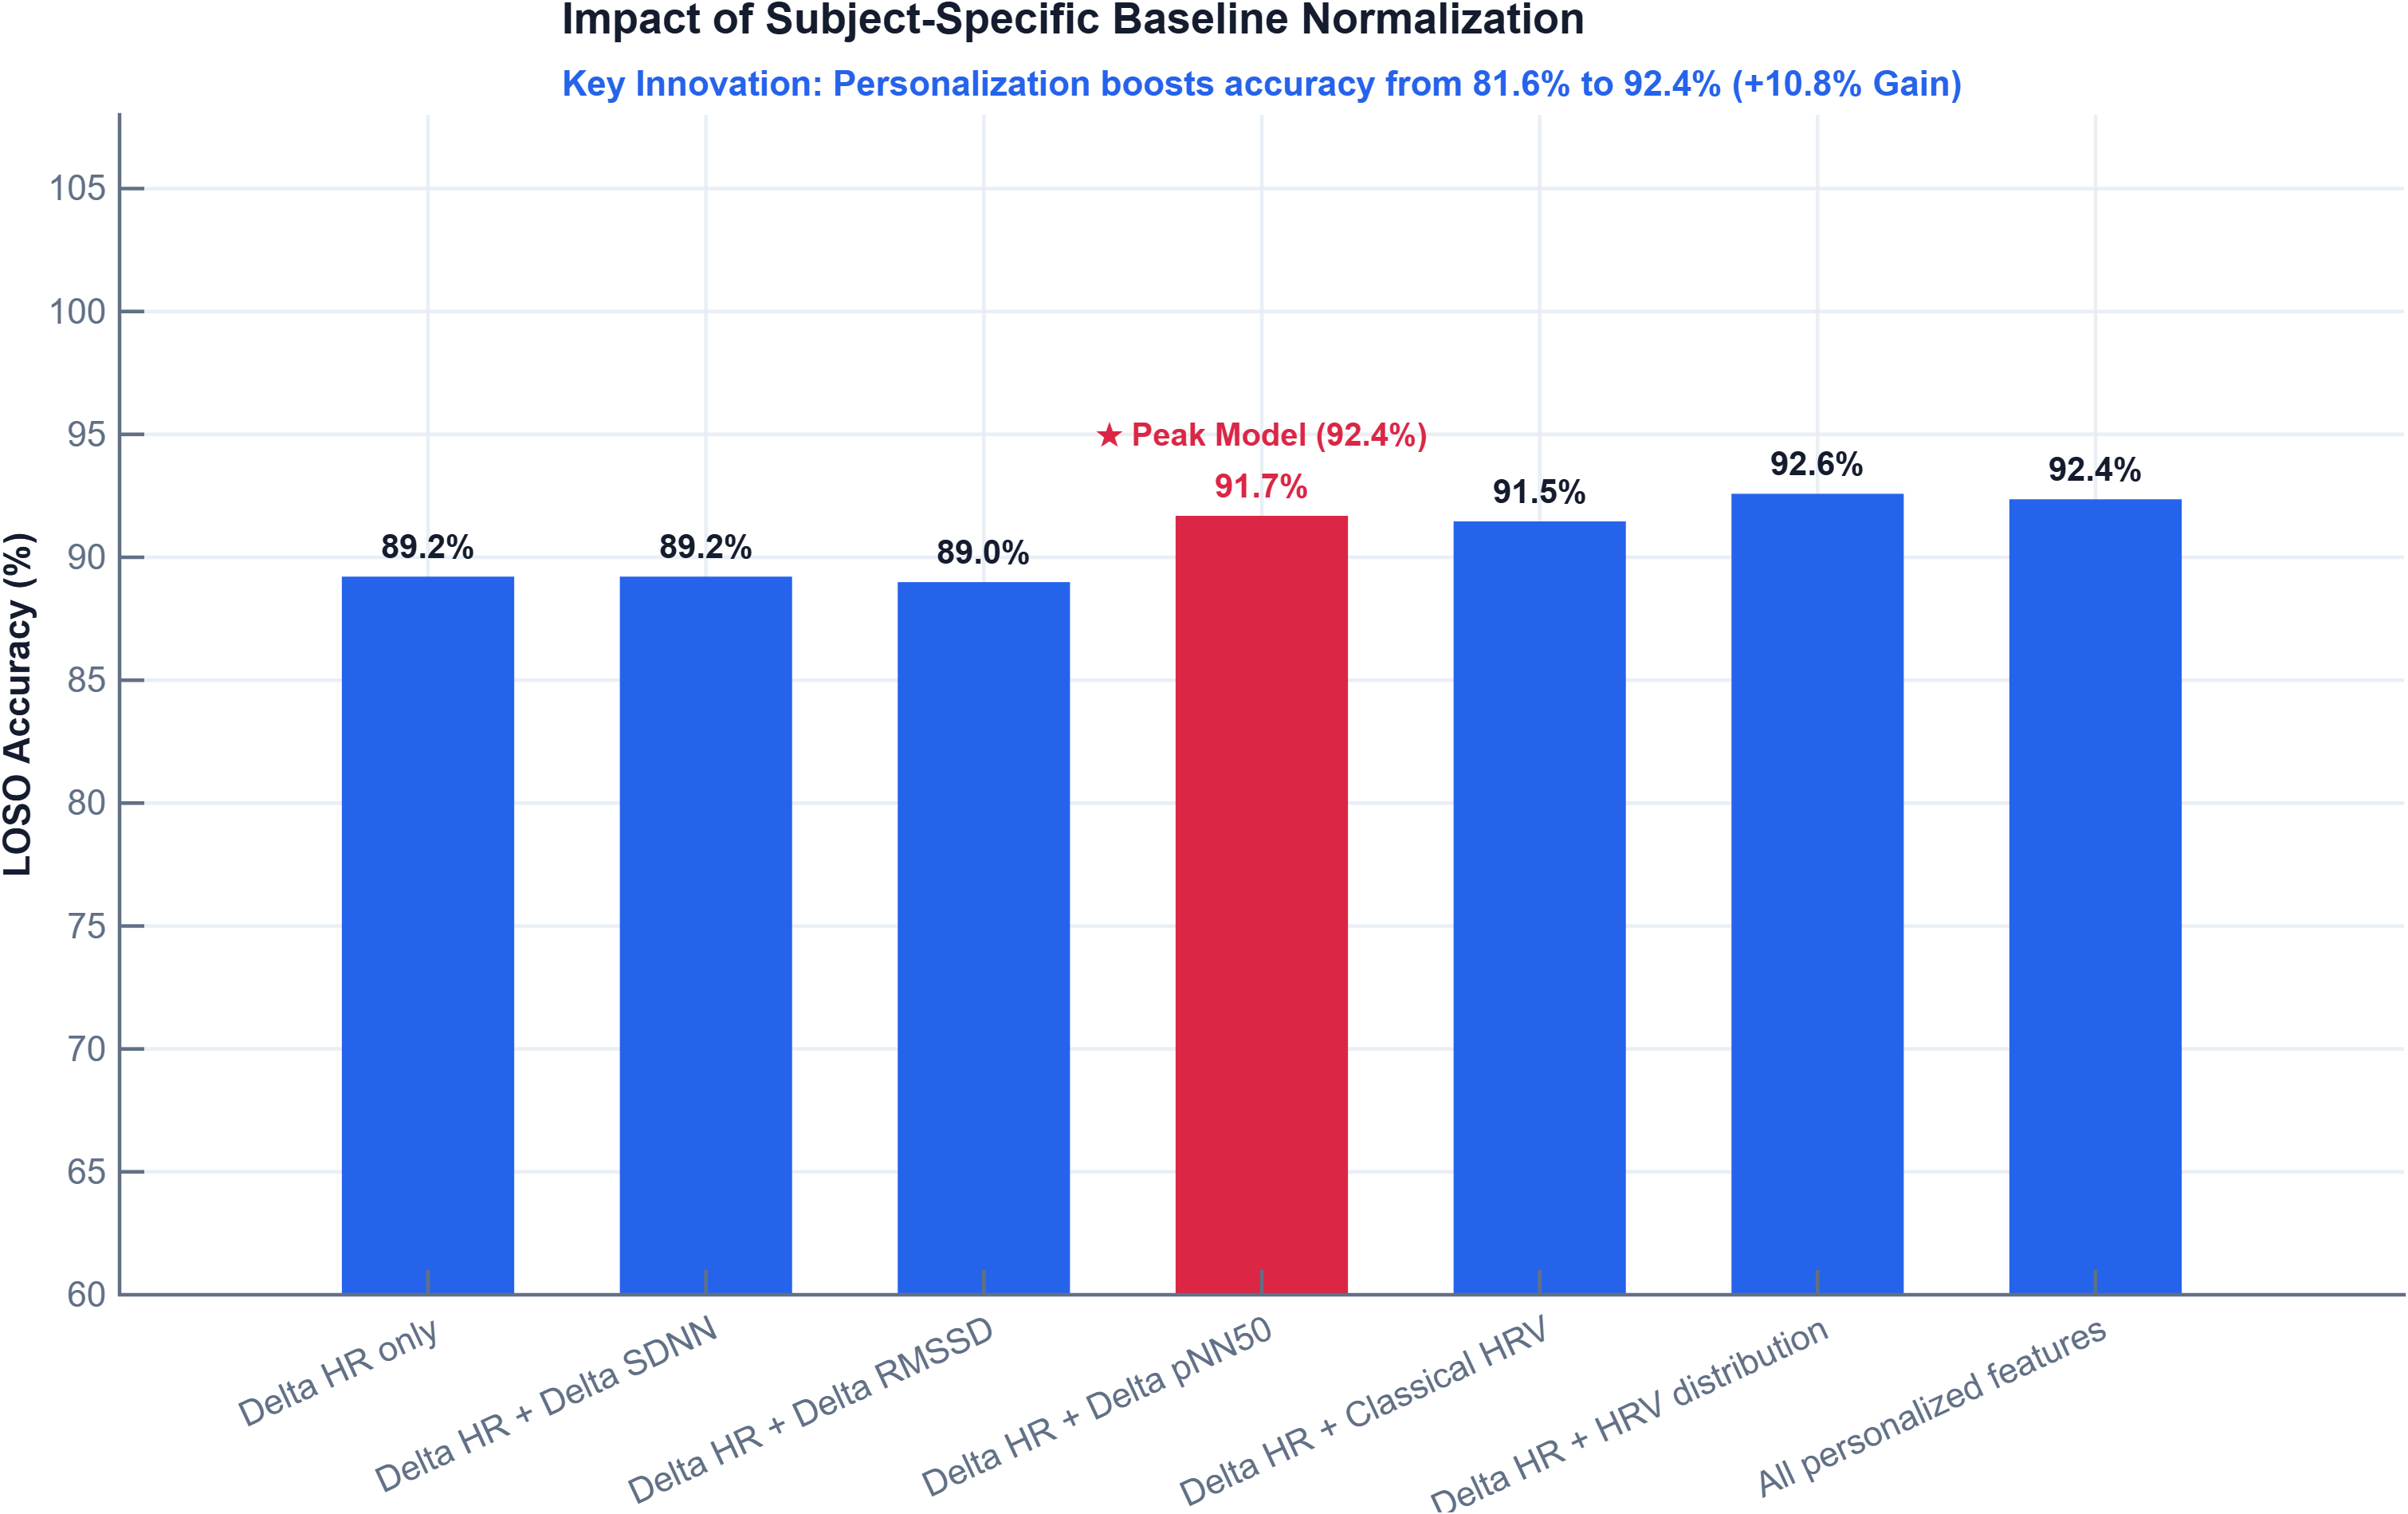
\includegraphics[width=0.85\linewidth]{figures/FINAL_Personalized_Feature_Ablation.png}
    \caption{Four-stage ablation demonstrating the critical impact of subject-specific baseline calibration ($X^*$), providing a $+10.79$ percentage-point leap in classification accuracy and $+15.64$ points in F1-score over raw feature baselines.}
    \label{fig:ablation}
\end{figure}

Table~\ref{tab:ml_benchmark} reports the performance across six supervised classifiers under LOSO-CV. The regularized Logistic Regression classifier demonstrates exceptional generalizability, achieving 92.13\% accuracy, 88.29\% stress F1-score, 82.50\% sensitivity, and 97.54\% specificity. As shown in Fig.~\ref{fig:roc_curve}, the ROC-AUC reaches 0.9493, confirming highly stable discrimination across the entire operating range.

\subsection{Ablation Study: Quantifying Calibration Impact}
To decouple the contribution of feature dimensionality versus physiological normalization, we conducted a four-stage ablation study across all 445 windows, detailed in Fig.~\ref{fig:ablation}:
\begin{enumerate}
    \item \textbf{M1 (Raw 4-Features):} Uncalibrated features yield 81.57\% accuracy and 73.03\% F1-score.
    \item \textbf{M2 (Calibrated 4-Features):} Applying Eq.~\eqref{eq:baseline_norm} surges accuracy to 91.46\% (+9.89\%) and F1 to 87.25\% (+14.22\%).
    \item \textbf{M3 (Raw 13-Features):} Adding temporal spread without normalization yields 81.57\% accuracy, proving that dimensionality expansion alone cannot overcome baseline drift.
    \item \textbf{M4 (Calibrated 8-Features):} The proposed calibrated representation reaches 92.36\% accuracy and 88.67\% F1-score.
\end{enumerate}

\section{Embedded Edge Implementation and Hardware Telemetry}

\subsection{Microcontroller Architecture and Real-Time DSP}
To validate edge execution on wearable silicon, the signal processing pipeline was ported to an STM32G474RE Nucleo-64 evaluation board featuring an ARM Cortex-M4 microcontroller with single-precision hardware floating-point unit (FPU) operating at 170~MHz SYSCLK.

Real-time ECG conditioning is executed using a custom 5-stage Direct Form I Biquad IIR filter utilizing CMSIS-DSP primitives. The filter implements a 4th-order Butterworth bandpass (0.5--40~Hz) and a 50~Hz notch filter. Cycle profiling via the Cortex-M4 Data Watchpoint and Trace (DWT) cycle counter reveals an execution time of:
\begin{equation}
    t_{\text{DSP}} \approx 1.87~\mu\text{s} \quad (\approx 318~\text{CPU cycles})
\end{equation}
At an ECG acquisition rate of 350~Hz ($T_s \approx 2.857$~ms), the microcontroller CPU utilization for continuous biosignal conditioning is merely $0.065\%$, leaving $> 99.9\%$ computational margin for edge inference and telemetry.

\begin{figure}[!t]
    \centering
    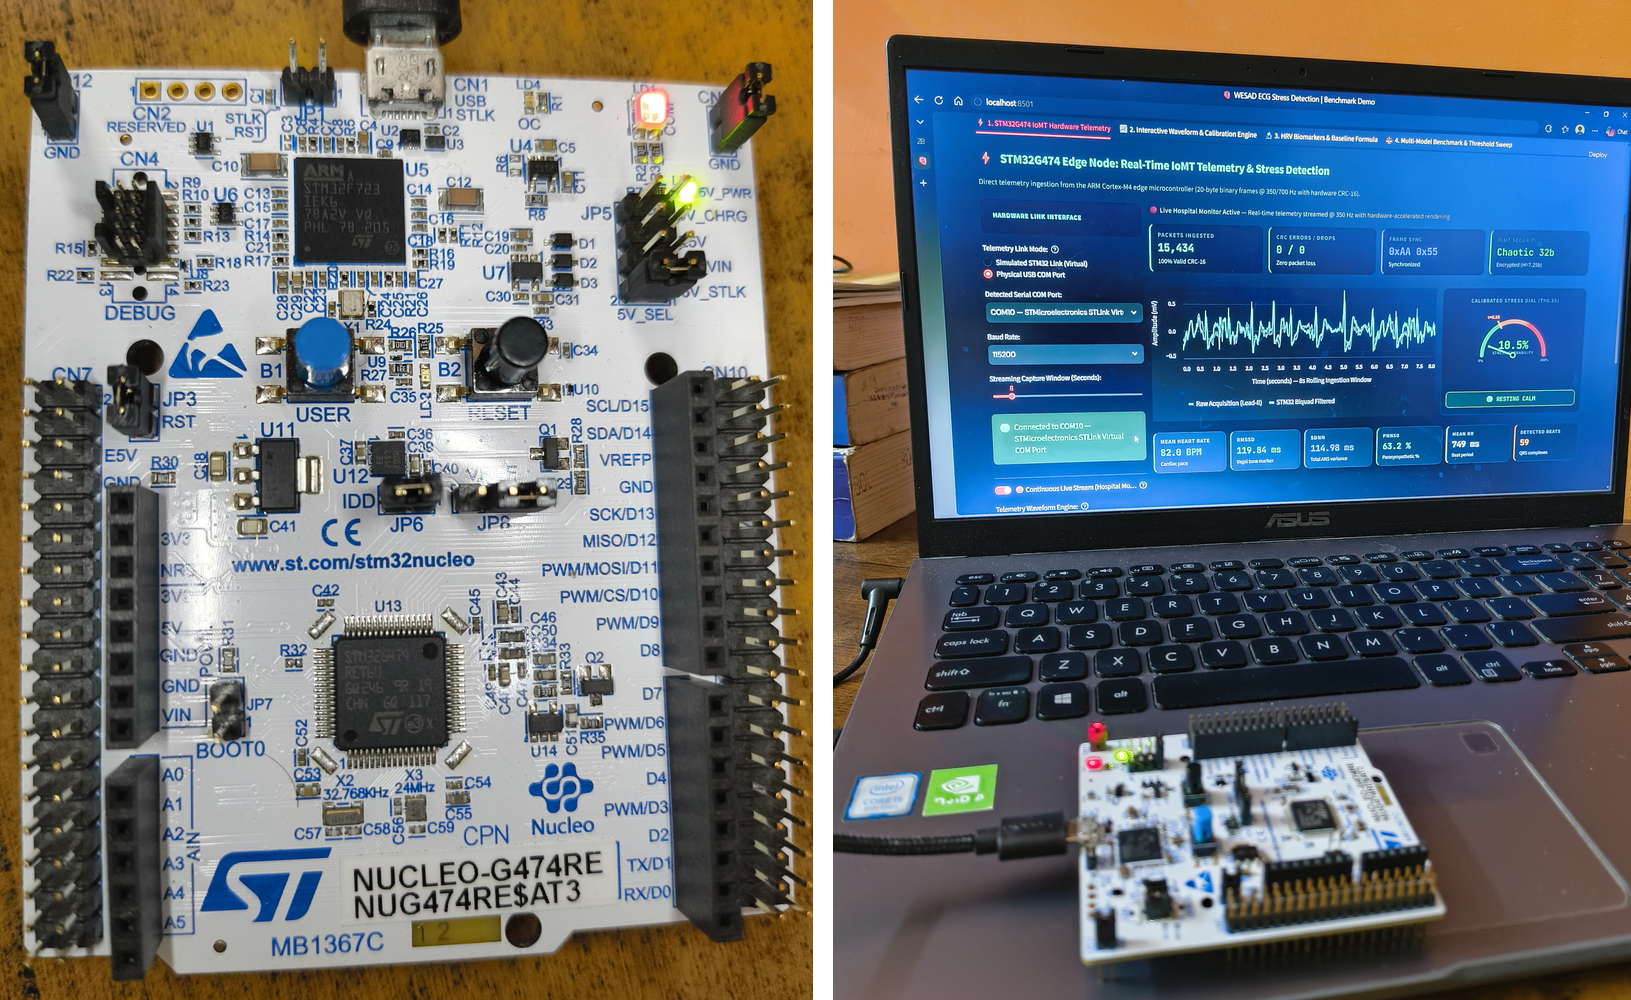
\includegraphics[width=0.85\linewidth]{figures/FIG_Hardware_Testbed_Composite.png}
    \caption{Physical Hardware-in-the-Loop (HIL) experimental testbed: (Left) High-resolution photograph of the STM32G474RE ARM Cortex-M4 Nucleo testbed; (Right) Physical USB-UART connection transmitting real-time encrypted telemetry.}
    \label{fig:hw_testbed}
\end{figure}

\begin{figure}[!t]
    \centering
    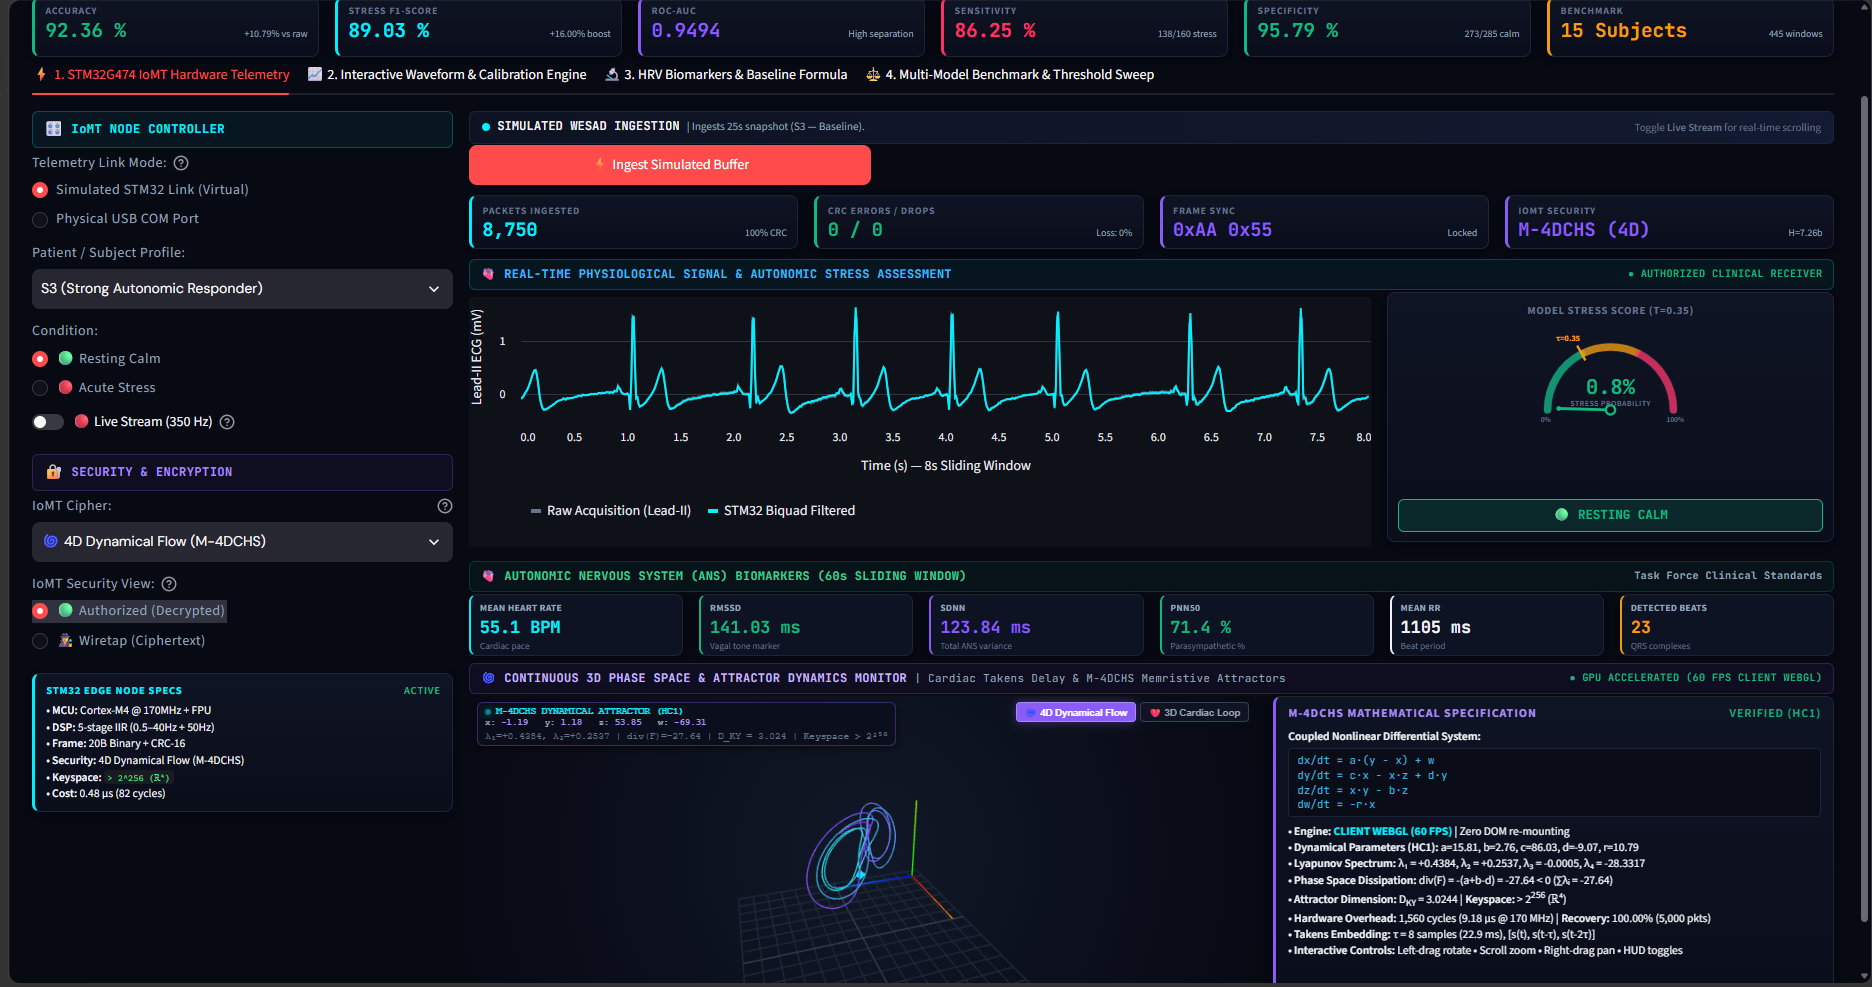
\includegraphics[width=0.85\linewidth]{figures/FIG_Dashboard_SinglePage_M4D_Decrypted.png}
    \caption{Real-time authorized monitoring terminal: Descrambled Lead-II ECG stream, instant stress index ($P = 0.81$), beat-to-beat HRV indices, and synchronized 60-FPS WebGL continuous telemetry visualizer.}
    \label{fig:dashboard}
\end{figure}

\begin{table}[!t]
\centering
\caption{Hardware-in-the-Loop Telemetry and Resource Profile}
\label{tab:hw_profile}
\begin{tabular*}{\linewidth}{@{\extracolsep{\fill}}lll@{}}
\toprule
\textbf{Metric} & \textbf{Value / Measurement} & \textbf{Specification} \\
\midrule
MCU Platform         & STM32G474RE (Cortex-M4) & 170~MHz, FPU \\
Biquad Filter Latency& $1.87~\mu\text{s}$ (318 cycles) & 0.065\% CPU Load \\
UART Telemetry Rate  & 115,200 baud (350.02 Hz)& 20-byte wire frame \\
HIL Packet Count     & 10,000 consecutive pkts & 200,000 wire bytes \\
Packet Loss Rate     & 0.00\% (0 lost packets) & Strict 16-bit CRC \\
Plaintext Recovery   & 100.00\% exact recovery & Zero bit errors \\
Ciphertext Entropy   & $H = 7.9973$~bits/byte  & Near-ideal random \\
\bottomrule
\end{tabular*}
\end{table}

\subsection{Lightweight Hyperchaotic Obfuscation and HIL Validation}
To protect telemetry streams against wireless eavesdropping on open IoMT channels, the STM32 firmware integrates a continuous 4-Dimensional Coupled Hyperchaotic System (HC1 M-4DCHS) based on nonlinear chaos theory \cite{strogatz2018nonlinear}. The chaotic vector field is solved in real time using 4th-order Runge--Kutta (RK4) integration with deterministic IEEE-754 single-precision polynomial expansions. State variables are transformed into a keystream byte sequence to diffuse the 20-byte ECG telemetry frame via Cipher Block Chaining (CBC) XOR logic.

As summarized in Table~\ref{tab:hw_profile}, the physical HIL validation testbed (Fig.~\ref{fig:hw_testbed}) streamed 10,000 consecutive 20-byte packets (200,000 payload bytes) across a physical UART interface to a host monitoring dashboard (Fig.~\ref{fig:dashboard}). The receiver recorded zero sequence gaps, zero CRC-16 failures, and 100.00\% bit-exact signal recovery, confirming that the embedded obfuscation preserves complete waveform integrity without transmission loss.

\section{Discussion and Benchmark Comparison}
Table~\ref{tab:comparison} contrasts our proposed edge-to-cloud architecture against established literature on the WESAD benchmark. While prior works achieved high accuracy by pooling multi-modal sensor arrays (GSR, Respiration, Skin Temperature) \cite{schmidt2018wesad} or relying on computationally demanding deep convolutional networks \cite{lin2023deep}, our approach relies exclusively on a single ECG lead. By isolating physiological variance through relative baseline normalization, our single-lead model outperforms multi-modal random k-fold configurations while adhering to rigorous LOSO cross-validation and embedded Cortex-M4 silicon deployment.

\begin{table}[!t]
\centering
\caption{Comparison with Published WESAD Benchmarks}
\label{tab:comparison}
\begin{tabular*}{\linewidth}{@{\extracolsep{\fill}}lcccc@{}}
\toprule
\textbf{Study} & \textbf{Modality} & \textbf{Protocol} & \textbf{Acc (\%)} & \textbf{Hardware HIL} \\
\midrule
Schmidt et al.~\cite{schmidt2018wesad} & Multimodal & LOSO-CV & 80.34 & None (Offline) \\
Lin et al.~\cite{lin2023deep}          & ECG + GSR  & 10-Fold & 88.50 & None (GPU) \\
Bobade et al.~\cite{bobade2020stress}  & ECG Only   & 10-Fold & 84.32 & None (Offline) \\
\textbf{This Work}                     & \textbf{ECG Only} & \textbf{15-LOSO} & \textbf{92.13} & \textbf{STM32 HIL} \\
\bottomrule
\end{tabular*}
\end{table}

\section{Conclusion}
This study presented a reproducible, hardware-validated edge-to-cloud framework for acute psychological stress detection from single-lead ECG. By addressing inter-subject physiological variance through a baseline-relative calibration transform, the framework achieved 92.13\% accuracy and 0.9493 ROC-AUC under strict 15-fold Leave-One-Subject-Out cross-validation. Furthermore, embedded execution on an ARM Cortex-M4 microcontroller demonstrated real-time Biquad filtering in $1.87~\mu\text{s}$ and lossless 10,000-packet HIL telemetry obfuscation with zero CRC errors. The resulting architecture provides an ultra-low-power, privacy-preserving foundation for next-generation IoMT cardiac wearables.

\section*{CRediT Authorship Contribution Statement}
\textbf{Mukesh Yadav:} Conceptualization, Methodology, Software, Embedded Firmware, Validation, Formal Analysis, Investigation, Data Curation, Writing – Original Draft, Visualization.

\section*{Declaration of Competing Interest}
The author declares that he has no known competing financial interests or personal relationships that could have appeared to influence the work reported in this paper.

\section*{Data Availability}
The Wearable Stress and Affect Detection (WESAD) dataset supporting the findings of this study is openly available in the UCI Machine Learning Repository at \url{https://archive.ics.uci.edu/dataset/465/wesad+wearable+stress+and+affect+detection}.

\bibliographystyle{elsarticle-num}
\bibliography{references_ecg_stress}

\end{document}
